\documentclass[12pt]{article}
\usepackage[a4paper]{geometry}
\usepackage[myheadings]{fullpage}
\usepackage{fancyhdr}
\usepackage{lastpage}
\usepackage{graphicx, wrapfig, subcaption, setspace, booktabs}
\usepackage[T1]{fontenc}
\usepackage[font=small, labelfont=bf]{caption}
\usepackage{fourier}
\usepackage[protrusion=true, expansion=true]{microtype}
\usepackage[spanish]{babel}
\usepackage{sectsty}
\usepackage{url, lipsum}
\usepackage{graphicx}
\usepackage[utf8]{inputenc}
\usepackage{courier}
\usepackage{ulem}
\usepackage{spverbatim}
\usepackage{multirow} %para las tablas
\usepackage{color}
\usepackage{graphicx}
\usepackage{epsfig}
\usepackage{multirow}
\usepackage{colortbl}
\usepackage{xcolor}
\usepackage{float}
\usepackage{hyperref}

\usepackage{adjustbox}
\usepackage{amsmath}
\usepackage{titlesec}

\setcounter{secnumdepth}{4}

\titleformat{\paragraph}
{\normalfont\normalsize\bfseries}{\theparagraph}{1em}{}
\titlespacing*{\paragraph}
{0pt}{3.25ex plus 1ex minus .2ex}{1.5ex plus .2ex}
\usepackage{listings} %For code in appendix
\lstset
{ %Formatting for code in appendix
    language=Matlab,
    basicstyle=\footnotesize,
    numbers=left,
    stepnumber=1,
    showstringspaces=false,
    tabsize=4,
    breaklines=true,
    breakatwhitespace=false,
}

\newcommand{\HRule}[1]{\rule{\linewidth}{#1}}
\onehalfspacing
\setcounter{tocdepth}{5}
\setcounter{secnumdepth}{5}

%-------------------------------------------------------------------------------
% HEADER & FOOTER
%-------------------------------------------------------------------------------
\pagestyle{fancy}
\fancyhf{}
\setlength\headheight{15pt}
\fancyhead[R]{PROGRAMACIÓN}
\fancyfoot[R]{\thepage}
%-------------------------------------------------------------------------------
% TITLE PAGE
%-------------------------------------------------------------------------------

\begin{document}

\title{ \normalsize \textsc{PROGRAMACIÓN}
		\\ [2.0cm]
		\HRule{2pt} \\
		\LARGE \textbf{\uppercase{Proyecto Proyectos}}
		\HRule{2pt} \\ [0.5cm] \bigskip
		\normalsize \today \vspace*{1\baselineskip}}

\date{}

\author{
        \emph{Autores:} \\ \\
		Xabier Garrote }

\maketitle
\newpage
\tableofcontents
\newpage


%--------------------------------------------------------------------% Las partes del documento de aqui en adelante ----------------------------------------------------------------------
\section{Objetivo del programa}
Facilitar la tarea de mecanizar los servicios de una empresa
\newpage
\section{Menú principal}
Es el menú que aparece nada mas iniciar el programa. Este menú se ha sido implementado con punteros a funciones. La pantalla del menú se ha intentado que sea lo mas parecida a la descrita en el enunciado.
\newpage
\section{Menú clientes}
Es una de las opciones del programa en la cual el usuario puede hacer diferentes tareas como dar de alta,modificar y consultar un cliente. El fichero donde se guarda los clientes es un fichero con organización directa. 
\subsection{Altas}
El programa intenta abrir el fichero en modo lectura escritura. Si no lo consigue abrirlo en este modo supondrá que no hay ningún cliente insertado aun. Por lo tanto intentara abrir el archivo en modo escritura. Si no lo consiguiera abrir de este modo diría un mensaje de error. Después de abrir el fichero calcularía el tamaño del fichero. A partir de calcular el tamaño del fichero lo dividiría por sizeof(reg) para saber cual es la posición del siguiente cliente. Después pediría por pantalla al usuario que insertara los datos del cliente. El programa pedirá confirmación para guardar el registro en el fichero. Si la respuesta fuera afirmativa. El programa se  posicionara en el fichero ya que conoce la posición a donde insertar el registró previamente calculada. Para finalizar el programa procederá a insertar el registro en el fichero y volverá al menú clientes.
\subsection{Modificar}
El programa intenta abrir el fichero en modo lectura escritura. Si no consiguiera abrirlo daría un mensaje de error. Después de abrir el fichero preguntara por que numero de cliente desea modificar. Si el numero de cliente insertado no esta entre los existentes, el programa mostraría un mensaje de error. Si el numero de cliente existe. El programa se posicionara en el fichero y leerá los datos de ese cliente. Después de leer los datos mostraría pantalla de modificación de datos para que el usuario pueda ir modificando los datos que desee. Una vez seleccione la opción salir de la pantalla de modificación de datos. El programa grabara los datos modificados en el fichero y volverá al menú clientes.
\subsection{Consultar}
El programa intenta abrir el fichero en modo lectura. Si no consiguiera abrirlo daría un mensaje de error. Después de abrir el fichero preguntara por que numero de servicio desea consultar. Si el numero de cliente insertado no existe, el programa mostraría un mensaje de error. Si el numero de cliente existe el programa leería los datos del fichero y los mostraría. Esperando a que el usuario le de intro para continuar y volver al menú clientes.
\newpage
\section{Menú servicios}
Es una de las opciones del programa en la cual el usuario puede hacer diferentes tareas como dar de alta,modificar y consultar un servicio. El fichero donde se guarda los servicios es un fichero con organización directa.
\subsection{Altas}
El programa intenta abrir el fichero en modo lectura escritura. Si no lo consigue abrirlo en este modo supondrá que no hay ningún servicio insertado aun. Por lo tanto intentara abrir el archivo en modo escritura. Si no lo consiguiera abrir de este modo diría un mensaje de error. Después de abrir el fichero calcularía el tamaño del fichero. A partir de calcular el tamaño del fichero lo dividiría por sizeof(reg) para saber cual es la posición del siguiente servicio. Después pediría por pantalla al usuario que insertara los datos del servicio. El programa pedirá confirmación para guardar el registro en el archivo. Si la respuesta fuera afirmativa. El programa se  posicionara en el fichero, ya que conoce la posición a donde insertar el registró previamente calculada. Para finalizar el programa procederá a insertar el registro en el fichero y volverá al menú servicios.
\subsection{Modificar}
El programa intenta abrir el fichero en modo lectura escritura. Si no consiguiera abrirlo daría un mensaje de error. Después de abrir el fichero preguntara por que numero de servicio desea modificar. Si el numero de servicio insertado no existe, el programa mostraría un mensaje de error. Si el numero de servicio existe. El programa se posicionara en el fichero y leerá los datos de ese cliente. Después de leer los datos mostraría pantalla de modificación de datos para que el usuario pueda ir modificando los datos que desee. Una vez seleccione la opción salir de la pantalla de modificación de datos. El programa grabara los datos modificados en el fichero y volverá al menú servicios.
\subsection{Consultar}
El programa intenta abrir el fichero en modo lectura. Si no consiguiera abrirlo daría un mensaje de error. Después de abrir el fichero preguntara por que numero de servicio desea modificar. Si el numero de servicio insertado no existe, el programa mostraría un mensaje de error. Si el numero de servicio existe el programa leería los datos del fichero y los mostrara. Esperando a que el usuario le de intro para continuar y volver al menu servicios.

\newpage
\section{Estilo de programación}
El programa se ha intentado dividir las tareas grandes en tareas mas pequeñas. Usando el paradigma procedimental. Además como recomienda en el libro \textbf{\textit{clean code} }Los nombres de las funciones empiezan por verbo y los nombres de las variables por sustantivo.

Se ha intentado que los nombres de las funciones sean lo mas auto descriptivas posibles a fin de evitar comentarios innecesarios.

\newpage
\section{Manual de usuario del programa}
El programa se compone de las siguientes partes:
\subsection{El menú principal}
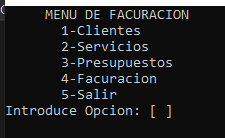
\includegraphics[]{MenuPrincipal.PNG}\\\\
En este menú el usuario tiene 4 opciones para elegir según la tarea que quiera hacer.
\subsubsection{Clientes}
Abre el menú clientes para poder gestionar los clientes.
\subsubsection{Servicios}
Abre el menú servicios para poder gestionar los servicios.
\subsubsection{Presupuestos}
Abriría la pantalla de de presupuestos. Esta opción no ha podido ser implementada debido a la falta de tiempo. Es por esta razón que muestra el siguiente mensaje al pulsar en ella.\\
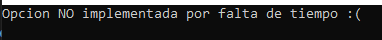
\includegraphics[]{OpcionNoImplementada.PNG} 
\subsubsection{Facturación}
Abriría la pantalla de facturación. Esta opción igual que la anterior no ha podido ser implementada debido a la falta de tiempo. Al pulsar en ella sale el siguiente mensaje:\\ 
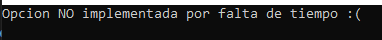
\includegraphics[]{OpcionNoImplementada.PNG}
\subsubsection{Salir}
Como su propio nombre indica es para salir del programa.

\subsection{Clientes}
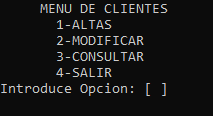
\includegraphics[]{MenuClientes.PNG}\\\\
En el menú clientes el usuario tiene tres opciones a elegir según la tarea que quiera llevar acabo.

\subsubsection{Altas}
Es para dar de alta a un nuevo cliente. Al pulsar en esta opción el programa se puede encontrar con dos casos diferentes.

\paragraph{1ºcaso}
Seria que todavía no se haya ningún cliente de alta. En este caso el programa crearía un nuevo fichero llamado "\textbf{clientes.dat}". Después de crear el fichero sacaría la pantalla de petición de datos poniendo el NºCliente 1 y pidiendo al usuario que inserte el resto de datos.\\\\
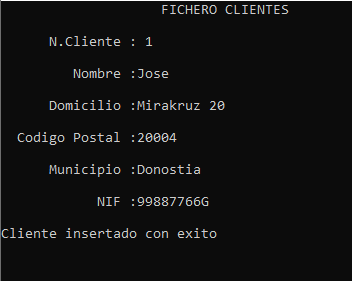
\includegraphics[]{PrimerClienteInsertado.PNG}\\\\
Después de leer los datos insertados por el usuario el programa preguntara pedirá conformación para guardar usuario. En caso de responder '\textbf{S}' el programa guardara el usuario.

\paragraph{2ºcaso}
Seria que haya clientes dados de alta de anterioridad. En este caso el programa calculara el numero del ultimo cliente en el fichero y le sumara uno. Después sacara la pantalla de petición de datos pidiendo al usuario que inserte el resto de datos.\\
Después de leer los datos insertado por el usuario el programa  pedira confirmacion y en caso de decir \textbf{S} grabara el registro al final del fichero y sacara mensaje por pantalla diciendo que el cliente se ha insertado correctamente.

\subsubsection{Modificar}
   Es para modificar los clientes que hay guardados. Al pulsar en esta opción el programa verifica si existe el fichero llamado "\textbf{clientes.dat}". Si no existiera daría un error indicando la no existencia del mismo. Si el fichero existe el programa pide que se introduzca un numero de cliente.\\
    
\includegraphics[]{PedirNumeroDeCliente.PNG}\\
    Depende el numero de cliente que se introduzca se pueden encontrar dos casos diferentes:
    \paragraph{1ºcaso}
    El numero de cliente introducido no existe en el fichero "\textbf{clientes.dat}". El programa mostraría el siguiente error.\\
    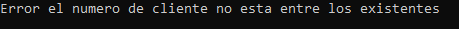
\includegraphics[]{ErrorNumeroClientesNoExistente.PNG}
    \paragraph{2ºcaso}
        El numero de cliente introducido existe en el fichero. A continuación aparecería la siguiente pantalla con los datos del cliente. Además el programa pedirá que dato desea modificar.\\
        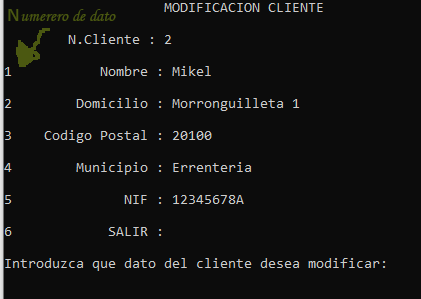
\includegraphics[]{ModificacionCliente.PNG}\\
        Una vez seleccionado el dato que se desea modificar el programa pedirá la nueva información. Si por ejemplo seleccionamos el dato 1 es decir modificar el nombre el programa nos mostrara lo siguiente:\\
        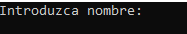
\includegraphics[]{ModificacionClienteIntroducirNombre.PNG}\\
        En el cual introduciremos el nuevo nombre y si todo a ido bien el programa nos mostrara un mensaje confirmando que el datos se ha modificado con éxito.\\
        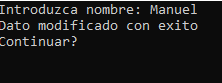
\includegraphics[]{ModificacionClienteNombreIntroducidoConExito.PNG}\\
        Después de darle a continuar el programa volverá a la pantalla anterior.\\
        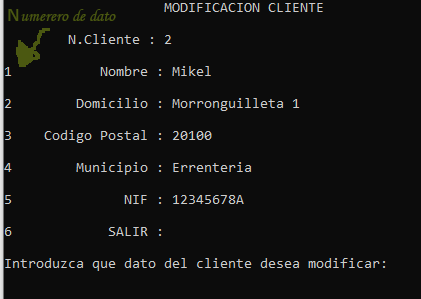
\includegraphics[]{ModificacionCliente.PNG}\\
        Esperando a que seleccionemos algún dato mas a modificar o que seleccionemos la opción 6 para salir.
\subsubsection{Consultar}
    Es para poder consultar los clientes que hay guardados. Si no hubiera ningún cliente guardado el programa daría un mensaje de error. Si hay clientes guardados el programa pedirá que se introduzca un numero de cliente.\\
    
\includegraphics[]{PedirNumeroDeCliente.PNG}\\
     Depende el numero de cliente que se introduzca se pueden encontrar dos casos diferentes:
     \paragraph{1ºcaso}
     El numero de cliente introducido no existe en el fichero. El programa mostraría el siguiente error.\\
    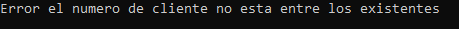
\includegraphics[]{ErrorNumeroClientesNoExistente.PNG}
    \paragraph{2ºcaso}
    El numero de cliente introducido existe en el fichero. Entonces el programa mostraría una pantalla como la siguiente enseñando los datos del respectivo cliente.\\
    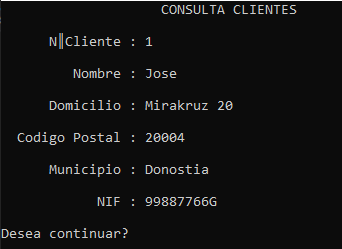
\includegraphics[]{PantallaConsultaClientesMostrandoCliente.PNG}\\
    Esperando a que se le de a la tecla intro para volver al menú clientes.
\subsubsection{Salir}
    Es para salir del menú clientes y volver al menú principal.
\subsection{Servicios}
En el menú servicios el usuario tiene tres opciones a elegir según la tarea que quiera llevar acabo.
\subsubsection{Altas}
Es para dar de alta a un nuevo servicio. Al pulsar en esta opción el programa se puede encontrar con dos casos diferentes.
\paragraph{1ºcaso}
Seria que todavía no se haya ningún servicio dado de alta. En este caso el programa crearía un nuevo fichero llamado "\textbf{servicios.dat}". Después de crear el fichero sacaría la pantalla de petición de datos poniendo el NºServicio 1 y pidiendo al usuario que inserte el resto de datos.\\\\
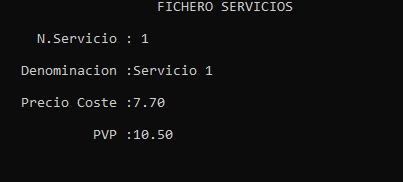
\includegraphics[]{PrimerServicioInsertado.PNG}\\\\
Después de leer los datos insertados por el usuario el programa pedira confirmacion y en caso de responder que \textbf{S} grabara los datos en el registro.

\paragraph{2ºcaso}
Seria que haya clientes dados de alta de anterioridad. En este caso el programa calculara el numero del ultimo cliente en el fichero y le sumara uno. Después sacara la pantalla de petición de datos pidiendo al usuario que inserte el resto de datos.\\
Después de leer los datos insertados por el usuario el programa pedira confirmacion y en caso de responder que \textbf{S} grabara los datos en el registro.

\subsubsection{Modificar}
   Es para modificar los servicios que hay guardados. Al pulsar en esta opción el programa verifica si existe el fichero llamado "\textbf{servicios.dat}". Si no existiera daría un error indicando la no existencia del mismo. Si el fichero existe el programa pide que se introduzca un numero de servicio.\\
    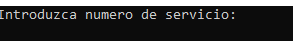
\includegraphics[]{PedirNumeroDeServicio.PNG}\\
    Depende el numero de servicio que se introduzca se pueden encontrar dos casos diferentes:
    \paragraph{1ºcaso}
    El numero de cliente introducido no existe en el fichero "\textbf{servicios.dat}". El programa mostraría el siguiente error.\\
    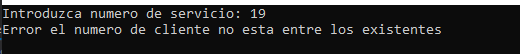
\includegraphics[]{ErrorNumeroDeServicioNoExiste.PNG}
    \paragraph{2ºcaso}
        El numero de servicio introducido existe en el fichero. A continuación aparecería la siguiente pantalla con los datos del servicio. Además el programa pedirá que dato desea modificar.\\
        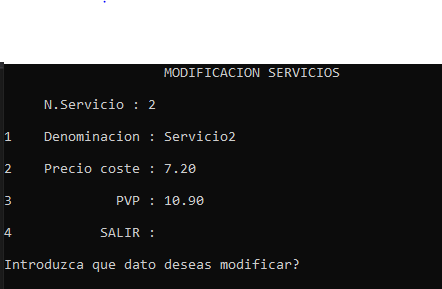
\includegraphics[]{ModificacionServicio.PNG}\\
        Una vez seleccionado el dato que se desea modificar el programa pedirá la nueva información. Si por ejemplo seleccionamos el dato 1 es decir modificar la denominación el  programa nos mostrara lo siguiente:\\
        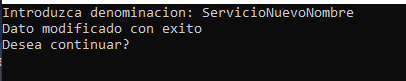
\includegraphics[]{ModificacionServicioIntroducirDenominacion.PNG}\\
        En el cual introduciremos el nuevo nombre y si todo a ido bien el programa nos mostrara un mensaje confirmando que el datos se ha modificado con éxito.\\
        Después de darle a continuar el programa volverá a la pantalla anterior.\\
        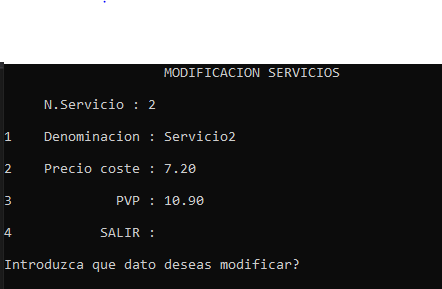
\includegraphics[]{ModificacionServicio.PNG}\\
        Esperando a que seleccionemos algún dato mas a modificar o que seleccionemos la opción 4 para salir.
        
    \subsubsection{Consultar}
    Es para poder consultar los servicios que hay guardados. Si no hubiera ningún servicio guardado el programa daría un mensaje de error. Si hay servicios guardados el programa pedirá que se introduzca un numero de servicio.\\
    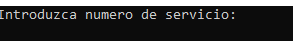
\includegraphics[]{PedirNumeroDeServicio.PNG}\\
     Depende el numero de servicio que se introduzca se pueden encontrar dos casos diferentes:
     \paragraph{1ºcaso}
     El numero de servicio introducido no existe en el fichero. El programa mostraría el siguiente error.\\
    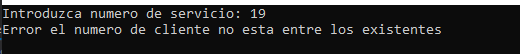
\includegraphics[]{ErrorNumeroDeServicioNoExiste.PNG}
    \paragraph{2ºcaso}
    El numero de servicio introducido existe en el fichero. Entonces el programa mostraría una pantalla como la siguiente enseñando los datos del respectivo servicio.\\
    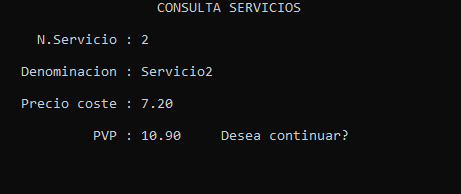
\includegraphics[]{PantallaConsultaServicioMostrandoServicio.PNG}\\
    Esperando a que se le de a la tecla intro para volver al menú servicios.
\subsubsection{Salir}
    Es para salir del menú servicios y volver al menú principal.
        


\end{document}